\chapter{Semantische analyse}
\label{ch:semantische_analyse}

Semantische analyse is het proces van een compiler dat:
\begin{itemize}
	\item definities van variabelen mapt op hun waarden,
	\item controleert dat elke expressie een correct type heeft,
	\item de abstract syntax tree omvormt zodat deze bruikbaar wordt om machinecode te genereren.
\end{itemize}

\section{Symbooltabellen}
\begin{lstlisting}[caption={Het scopeprobleem.},captionpos=b,label={code:symboltable_example}]
int b = 0;
extern int a;
void foobar(float b){
  if(b == 0.0){
    char * b = malloc(1);
    *b = 0;
  }
}
\end{lstlisting}

In code \protect\ref{code:symboltable_example} wordt er een nullbyte weggeschreven naar $b$. Is dit een string, float, 32 bit integer of 64 bit integer? Het algemene probleem is dat er verschillende scopes zijn, en binnen elke scope kan dezelfde variabele identifier gebruikt worden. Via \textbf{symbooltabellen} wordt dit efficiënt opgelost.
Een symbooltabel bestaat uit een \textbf{omgeving} $\sigma_i$ en een verzameling \textbf{bindings}:
$$\sigma_1 = \{g \mapsto string, a \mapsto int\}$$

Elke omgeving $\sigma_i$ bestaat uit de samenstelling van zijn specifieke bindings en eventueel de bindings van andere $\sigma_{j}$ voor $j \neq i$. De specifieke bindings van $\sigma_i$ hebben voorrang op de bindings van elke andere $\sigma_{j}$.

\begin{figure}[h]
	\centering
	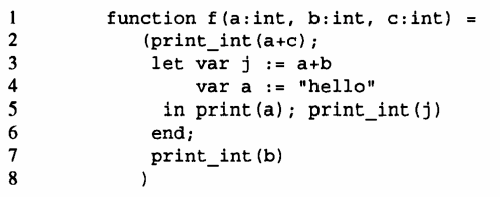
\includegraphics[width=\textwidth]{symbooltabellen_code}
	\caption{}
	\label{fig:symbooltabellen_code}
\end{figure}

De omgevingen kunnen voor de code uit figuur \ref{fig:symbooltabellen_code} gedefinieerd worden als:
\begin{equation*}
	\begin{split}
		\hbox{bestaande omgeving: } & \sigma_0 \\
		\hbox{functiedeclaratie: } & \sigma_1 = \sigma_0 + \{a \mapsto int, b \mapsto int, c \mapsto int\} \\ 
		\hbox{regel 3: } & \sigma_2 = \sigma_1 + \{j \mapsto int \} \\
		\hbox{regel 4: } & \sigma_3 = \sigma_2 + \{a \mapsto string \} \\
	\end{split}
\end{equation*}

\begin{itemize}
	\alert De $+$ operatie bij twee omgevingen is hier niet commutatief. De precieze betekenis hangt af van de scoping regels van een taal.
	\item Er zijn \underline{twee mogelijke implementaties}:
	\begin{itemize}
		\item \textbf{Imperatieve implementatie:} Er is slechts één omgeving $\sigma$ die aangepast wordt naar $\sigma_1$, $\sigma_2$, ... wanneer dit nodig is. Een \textbf{destructieve update} zal $\sigma_1$ vernietigen wanneer $\sigma_2$ vereist is, maar kan via de \textbf{undo stack} terug naar $\sigma_1$ gaan. Dit kan bijvoorbeeld geïmplementeerd worden met een hashtabel. De operatie $\sigma' = \sigma + \{a \mapsto \tau \}$ wordt geïmplementeerd door de sleutel $a$ met waarde $\tau$ toe te voegen aan de hashtabel. Om $\sigma$ te bekomen wordt de sleutel $a$ dan verwijderd. Dit werkt natuurlijk alleen als er toegevoegd wordt op een stacksgewijze manier.
		\item \textbf{Functionele implementatie:} In deze implementatie wordt de originele $\sigma$ onaangetast en wordt er een nieuwe datastructuur voor $\sigma'$ gemaakt. Dit kan ook met hashtabellen geïmplementeerd worden, maar wordt eerder met binaire zoekboomen, eventueel gebalanceerd, geïmplementeerd.
	\end{itemize}
\end{itemize}

\subsection{Efficiëntere symbooltabellen}
Er zijn een aantal manieren om symbooltabellen te verbeteren:
\begin{itemize}
	\item In plaats van strings bij te houden in de hashtabel of zoekboom kunnen er pointers bijgehouden worden. Dit vermijdt te veel stringoperaties.
	\item Een andere tabel houdt wel nog deze strings bij, waarnaar kan gerefereerd worden.
	\item Enkel tijdens het opbouwen van de tabellen wordt er met strings gewerkt.
	\item Stapel houdt scopes bij en aangemaakte symbolen bij \underline{imperatieve} tabellen:
	\begin{itemize}
		\item push \texttt{beginScope} bij binnengaan scope.
		\item push elk symbool bij declaratie in scope.
		\item bij verlaten van de scope: pop tot aan \texttt{beginScope}.
	\end{itemize}
\end{itemize}



\section{Type Checking}
Kijken of de gebruikte veranderlijken:
\begin{itemize}
	\item gedeclareerd zijn
	\item ze van het juiste type zijn
	\item of de types van expressies correct zijn
\end{itemize}
Door de abstract syntax tree in postorder te overlopen kan dit geïmplementeerd worden. Er zullen altijd eerst declaraties bezocht worden. Er zijn verschillende visitors voor zowel variabelen, expressies als declaraties:
\begin{lstlisting}
struct expty transVar(S_table venv, S_table tenv, A_var v);
struct expty transExp(S_table venv, S_table tenv, A_exp a);
void         transDec(S_table venv, S_table tenv, A_dec d);
struct Ty_ty transTy (              S_table tenv, A_ty a);
\end{lstlisting}
\subsection{Expressies}
Type Checking expressies wordt uitgevoerd op de abstract syntax tree. Er wordt gekeken of subexpressies het juiste type hebben, en bepalen dan ook het resulterende type.
\begin{lstlisting}
struct expty {Tr_exp exp; Ty_ty ty;};
struct expty expTy(Tr_exp exp, Ty_ty ty) {
  struct expty e; e.exp=exp; e.ty=ty; return e;
}

struct expty transExp(S_table venv, S_table tenv, A_exp a) {
  switch(a->kind) {
    case A_opExp: {
      A_oper oper = a->u.op.oper;
      struct expty left = transExp(venv, tenv, a->u.op.left);
      struct expty right = transExp(venv, tenv, a->u.op.right);
      if (oper == A_plusOp) {
        if(left.ty->kind != Ty_int)
          EM_error(a->U.op.left->pos, "integer required"); 
        if(right.ty->kind != Ty_int)
          EM_error(a->U.op.right->pos, "integer required");
        return expTy(NULL, Ty_int());
      }
    }
  }
}
\end{lstlisting}


\subsection{Variabelen}
De binding variabelen worden opgezocht in de symbooltabel. 
\begin{lstlisting}
struct expty transVar(S_table venv, S_table tenv, A_var v) {
  switch(v->kind) {
    case A_simpleVar: {
      E_enventry x = S_look(venv, v->u.simple);
      if(x && x->kind == E_varEntry)
        return expTy(NULL, actaul_ty(x->u.var.ty));
      else {
        EM_error(v->pos, "undefined variabele %s", S_name(v->u.simple));
        return expTy(NULL,Ty_int());
      }
    }
    case A_fieldVar: ...
  }
}
\end{lstlisting}
\subsection{Declaraties}

